\documentclass[conference]{IEEEtran}
\usepackage{cite}
\usepackage{amsmath,amssymb}
\usepackage{graphicx}
\graphicspath{{figs/}}
\usepackage{booktabs}
\usepackage[hidelinks]{hyperref}

\begin{document}

\title{Graph Neural Network Surrogates for a Coupled Heat-Conduction and
Pyrolysis Solver in Thermal Protection System Design}

\author{\IEEEauthorblockN{Grey Goodwin}
\IEEEauthorblockA{University of Kentucky \\
Lexington, KY, USA \\
grey.goodwin@uky.edu}}

\maketitle

\begin{abstract}
% DRAFT abstract from the white paper; tighten to ~150-200 words for IEEE.
Thermal protection system (TPS) design relies on repeated evaluation of an
expensive, coupled physics solver that resolves heat conduction, pyrolysis,
pyrolysis-gas transport, and aerothermal surface chemistry. We present early work
toward a graph neural network (GNN) surrogate that learns the per-step evolution
of a 1D heat-shield pyrolysis solver. As a foundation, we re-implement a trusted
Fortran reference solver in modular, vectorized Python and verify it against the
original by column-level comparison of its thermocouple and density outputs,
matching to machine precision on a conduction--pyrolysis case and to 0.064~K on a
full gas and aerothermal case. Training on data from the validated solver, a
per-cell message-passing GNN reproduces a held-out heating scenario over a full
60~s rollout to a mean error of 7.6~K and tracks the pyrolysis front to within a
fraction of a millimeter.
\end{abstract}

\begin{IEEEkeywords}
graph neural networks, surrogate models, thermal protection systems, pyrolysis,
scientific machine learning
\end{IEEEkeywords}

\section{Introduction}
% 1.1 TPS / heat-shield design problem
% 1.2 + 1.3 cost bottleneck and the surrogate response (CITE motivation \cite{...})
% 1.4 contribution and scope
% 1.5 relation to prior bead/Sod work (CITE own work \cite{...})
Thermal protection systems shield a vehicle from the intense aerothermal heating
of atmospheric entry. \emph{[draft body from white paper; add citations at marked
spots.]} Our surrogate follows the mesh-based graph-network line of
work~\cite{meshgraphnets,sanchez2020learning}, applied here to a multi-physics
heat-shield solver.

% Suggested citation anchors:
%  - surrogate motivation: \cite{surrogate_motivation}
%  - mesh-based GNN simulation: \cite{meshgraphnets,sanchez2020learning}
%  - TPS/ablation surrogates: \cite{tps_surrogate}
%  - prior LAUMeltFlow bead/Sod work: \cite{own_symposium}

\section{Reference Solver}
% Physics: conduction + pyrolysis + Darcy gas + aerothermal BC. Eq. (1).
\begin{equation}
\rho\, c_p\, \frac{\partial T}{\partial t}
  = \frac{\partial}{\partial x}\!\left(k\, \frac{\partial T}{\partial x}\right)
  + (\text{pyrolysis and gas source terms}).
\end{equation}

\section{Methodology}
\subsection{Python Port}
\subsection{Verification}
\subsection{Training-Data Generation}
\subsection{GNN Architecture}

\begin{figure}[t]
  \centering
  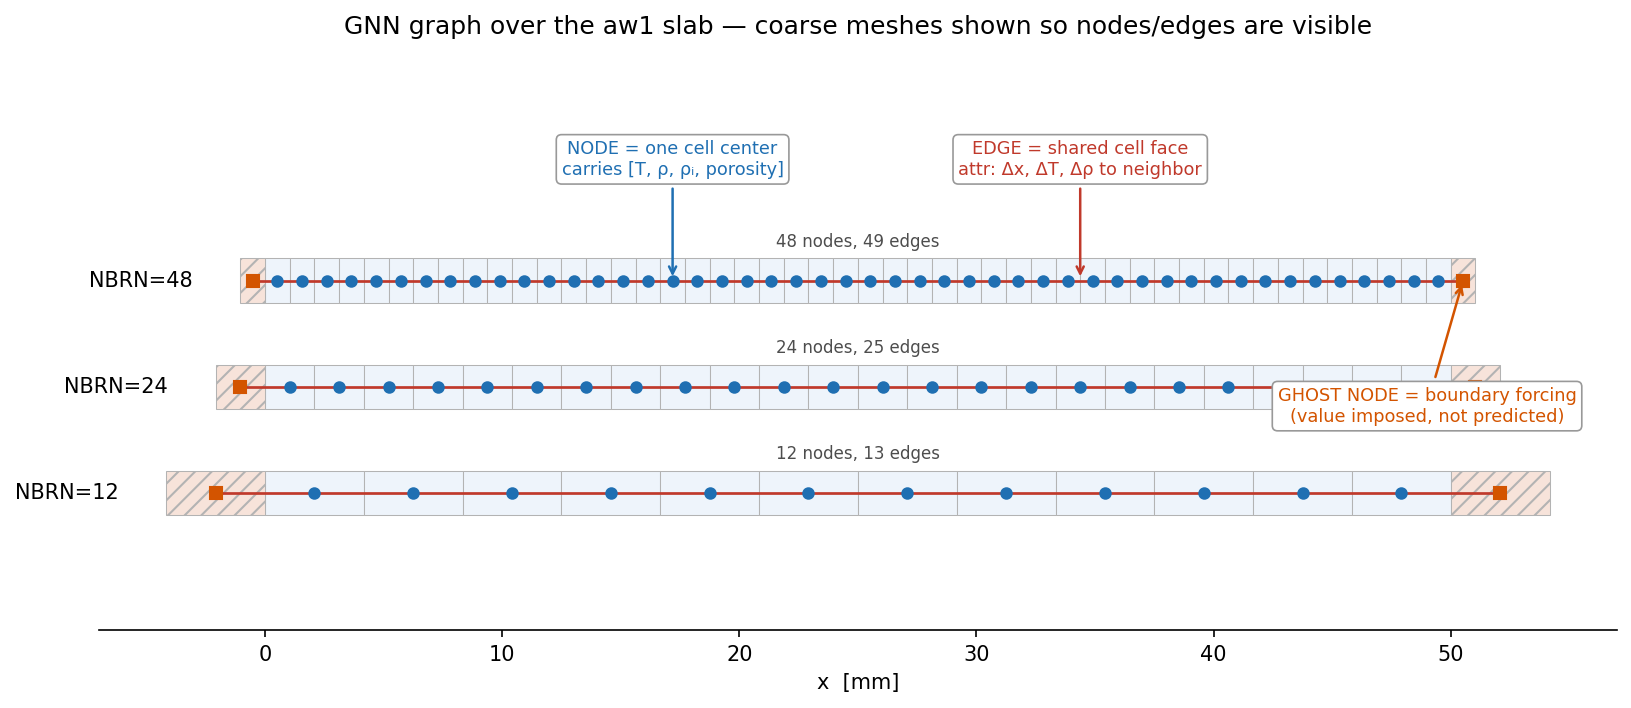
\includegraphics[width=\columnwidth]{graph.png}
  \caption{The mesh as a graph: each finite-volume cell is a node carrying
  $[T,\rho,\rho_i,\text{porosity}]$; edges join neighboring cells with relative
  features (neighbor-minus-self state and the cell spacing $\Delta x$). Ghost
  nodes at the ends impose the boundary forcing. Weights are shared across all
  cells. (Coarse meshes shown for legibility.)}
  \label{fig:graph}
\end{figure}

\section{Results}
\subsection{Port Validation}
% aw1 bit-exact; aw2_tc21 to 0.064 K. Table below.
\begin{table}[t]
\caption{Port validation against the Fortran reference (\texttt{aw2\_tc21}).}
\label{tab:val}
\centering
\begin{tabular}{ll}
\toprule
Quantity & Agreement \\
\midrule
All temperature columns & max 0.064~K, mean $\sim$$4\times10^{-4}$~K \\
Hot aerothermal surface & 0.06~K \\
Densities & $\sim$$10^{-3}$ to $10^{-9}$ \\
Time, cold back face & bit-exact \\
\bottomrule
\end{tabular}
\end{table}

\subsection{Surrogate Accuracy (aw1)}
% aw1: 7.6 K mean rollout (~0.5-1% of field); tracks pyrolysis front <1 mm.
% Multi-step (rollout) training cut end-of-traj error from 100s of K to 10s of K.

\begin{figure*}[t]
  \centering
  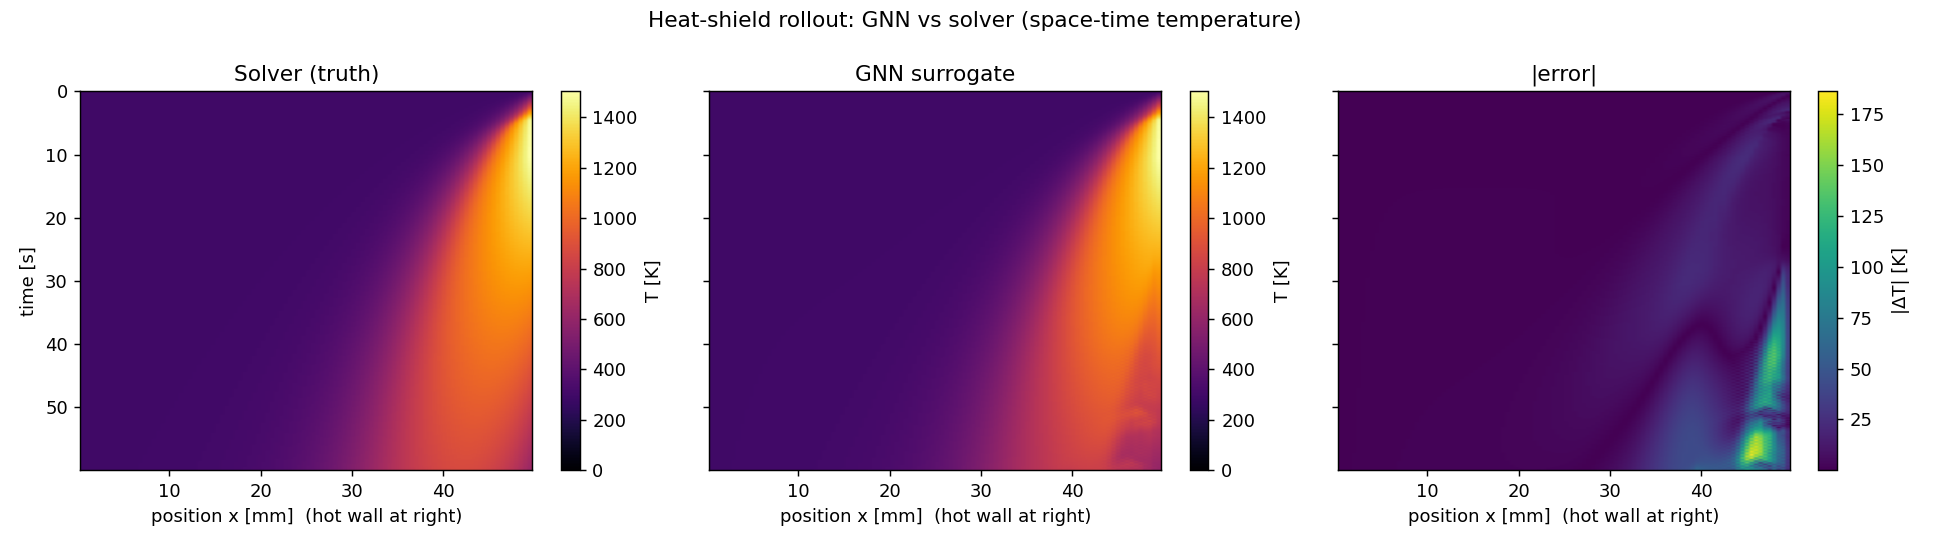
\includegraphics[width=\textwidth]{aw1_rollout_spacetime.png}
  \caption{aw1 surrogate rollout (gas off), space-time temperature: solver truth
  (left), GNN surrogate (center), absolute error (right). Mean rollout error
  7.6~K over the full 60~s; the surrogate field is visually indistinguishable from
  the solver and the error is small everywhere.}
  \label{fig:aw1rollout}
\end{figure*}

\subsection{Gas Case (aw2): A Diagnosed Failure Mode}
\label{sec:aw2}
% NEGATIVE result. In-sample bounded ~625 K, but HELD-OUT diverges (3587 K):
% the surrogate does not generalize across forcings on the gas case.
% Cause is TEMPORAL not spatial -- per-cell aw2 is gentler (111 vs 221 K), but the
% square-pulse aero flux jumps the surface 734 K per super-step (vs aw1's 41 K).
% dt-aware adaptive cadence + stay-put reg recover in-sample behavior but not held-out.
% Ruled out: more trajectories, gas-as-input, wider stencil. Solver verified sound.

\begin{figure*}[t]
  \centering
  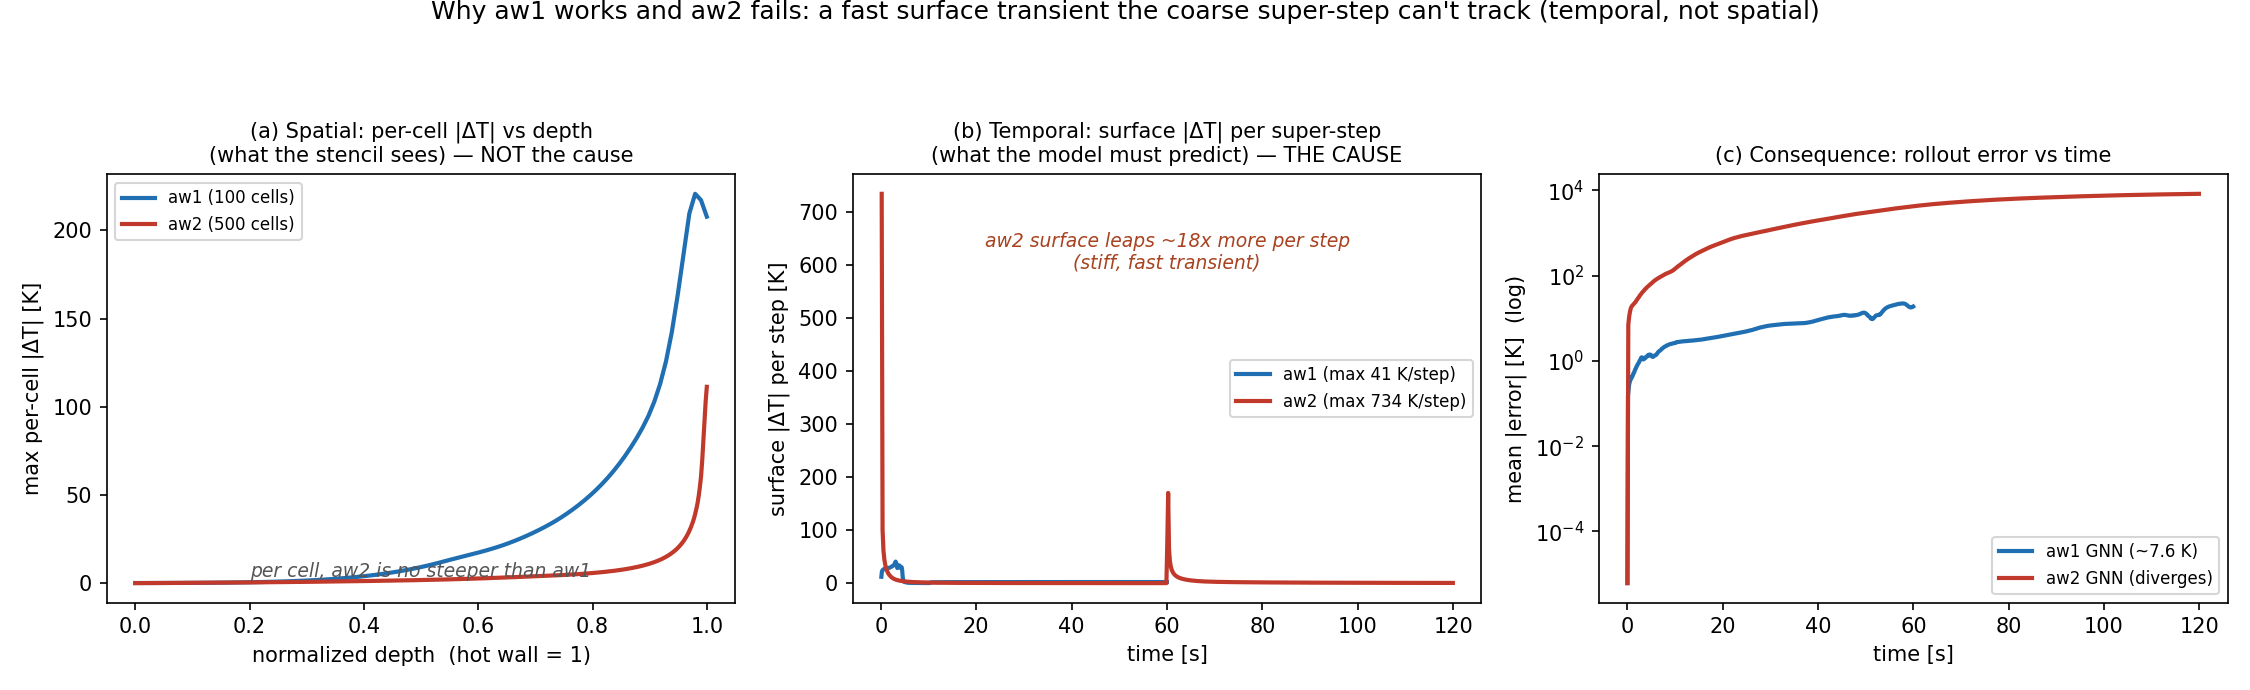
\includegraphics[width=\textwidth]{why_aw1_aw2.png}
  \caption{Why aw2 fails and aw1 does not, and why the cause is temporal not
  spatial. (a) Per-cell spatial $|\Delta T|$: aw2 is no steeper than aw1.
  (b) Per-super-step surface $|\Delta T|$: aw2 leaps $\sim$18$\times$ more
  (734 vs 41~K) under the square-pulse aerothermal flux. (c) The consequence:
  aw1 rollout error stays $\sim$7.6~K while aw2 diverges.}
  \label{fig:why}
\end{figure*}

\begin{figure}[t]
  \centering
  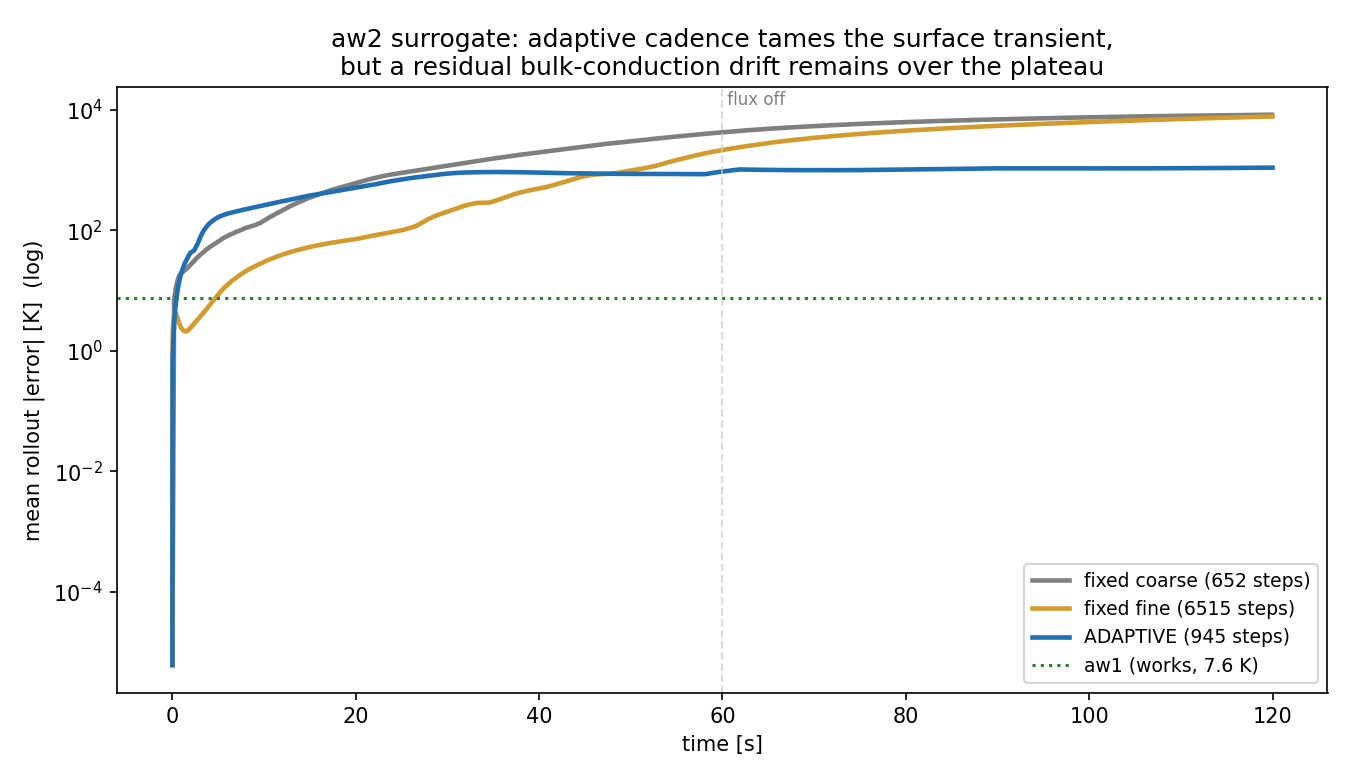
\includegraphics[width=\columnwidth]{aw2_progress.png}
  \caption{aw2 rollout error vs time across recipes. Fixed coarse and fixed fine
  cadence both diverge; the $\Delta t$-aware adaptive schedule stays bounded.
  All shown in-sample; held-out, even the adaptive model does not yet generalize
  (Section~\ref{sec:aw2}).}
  \label{fig:aw2prog}
\end{figure}

\subsection{Wall Time}
% Fortran ~3 min vs Python ~15.6 min (aw2_tc21). GNN ~4x faster than Python solver
% on aw1 (CPU); modest -- bigger super-step / mesh / amortization not yet exercised.

\section{Discussion}
% (1) aw1 success: mesh-native inductive bias; learns local dynamics + moving front.
% (2) The aw2 boundary, sharp and explainable: a fixed-step state-delta rollout is the
%     wrong vehicle for a fast localized forcing transient; in-sample-vs-held-out gap is
%     the honesty point -> motivates the conservative flux-form fix (Sec. Future Work).
% (3) Data-selection lesson: trajectory vs volume sampling; ablator's coupled T-char manifold.
% (4) Failure modes: rollout error accumulation (cf. bead paper), quiescent-cell bias.

\section{Future Work}
% Conservative flux-form GNN for the gas case: predict face fluxes -> divergence, so a
%   uniform field gives EXACTLY zero change -> kills the quiescent bias at the root.
%   Most promising route to an aw2 surrogate that generalizes.
% Mesh-resolution generalization (multi-res training). 2D/3D. Radiation + recession.

\section{Conclusion}

\section*{Acknowledgment}
This work builds on the reference heat-shield solver developed by Dr.\ Martin and
on a graph-neural-network surrogate program within the group.

\bibliographystyle{IEEEtran}
\bibliography{heat_gnn_refs}

\end{document}
